% -*- latex
%%%%%%%%%%%%%%%%%%%%%%%%%%%%%%%%%%%%%%%%%%%%%%%%%%%%%%%%%%%%%%%%
%%%%
%%%% This TeX file is part of the tutorial
%%%% `Introduction to the PETSc library'
%%%% by Victor Eijkhout, eijkhout@tacc.utexas.edu
%%%%
%%%% copyright Victor Eijkhout 2012-2020
%%%%
%%%%%%%%%%%%%%%%%%%%%%%%%%%%%%%%%%%%%%%%%%%%%%%%%%%%%%%%%%%%%%%%

\sectionframe{\texttt{Vec} datatype: vectors}

%\subsection{Basic stuff}

\begin{details}
\frame[containsverbatim]{
\frametitle{Create calls}
\small
Everything in PETSc is an object, with create and destroy calls:
\begin{verbatim}
VecCreate(MPI_Comm comm,Vec *v);
VecDestroy(Vec *v);

/* C */
Vec V;
VecCreate(MPI_COMM_SELF,&V);
VecDestroy(&V);

! Fortran
Vec V
call VecCreate(MPI_COMM_SELF,V,e)
call VecDestroy(V,e)
\end{verbatim}
Note: in Fortran there are no `star' arguments
}

\frame[containsverbatim]{\frametitle{More about vectors}
A vector is a vector of \n{PetscScalar}s: there are no vectors of
integers (see the \n{IS} datatype later)

The vector object is not completely created in one call:
\begin{verbatim}
VecSetType(V,VECMPI) // or VECSEQ
VecSetSizes(Vec v, int m, int M);
\end{verbatim}
Other ways of creating: make more vectors like this one:
\begin{verbatim}
VecDuplicate(Vec v,Vec *w);
\end{verbatim}

}
\end{details}

\frame[containsverbatim]{\frametitle{Parallel layout up to PETSc}
\begin{verbatim}
VecSetSizes(Vec v, int m, int M);
\end{verbatim}
Local size can be specified as \n{PETSC_DECIDE}.

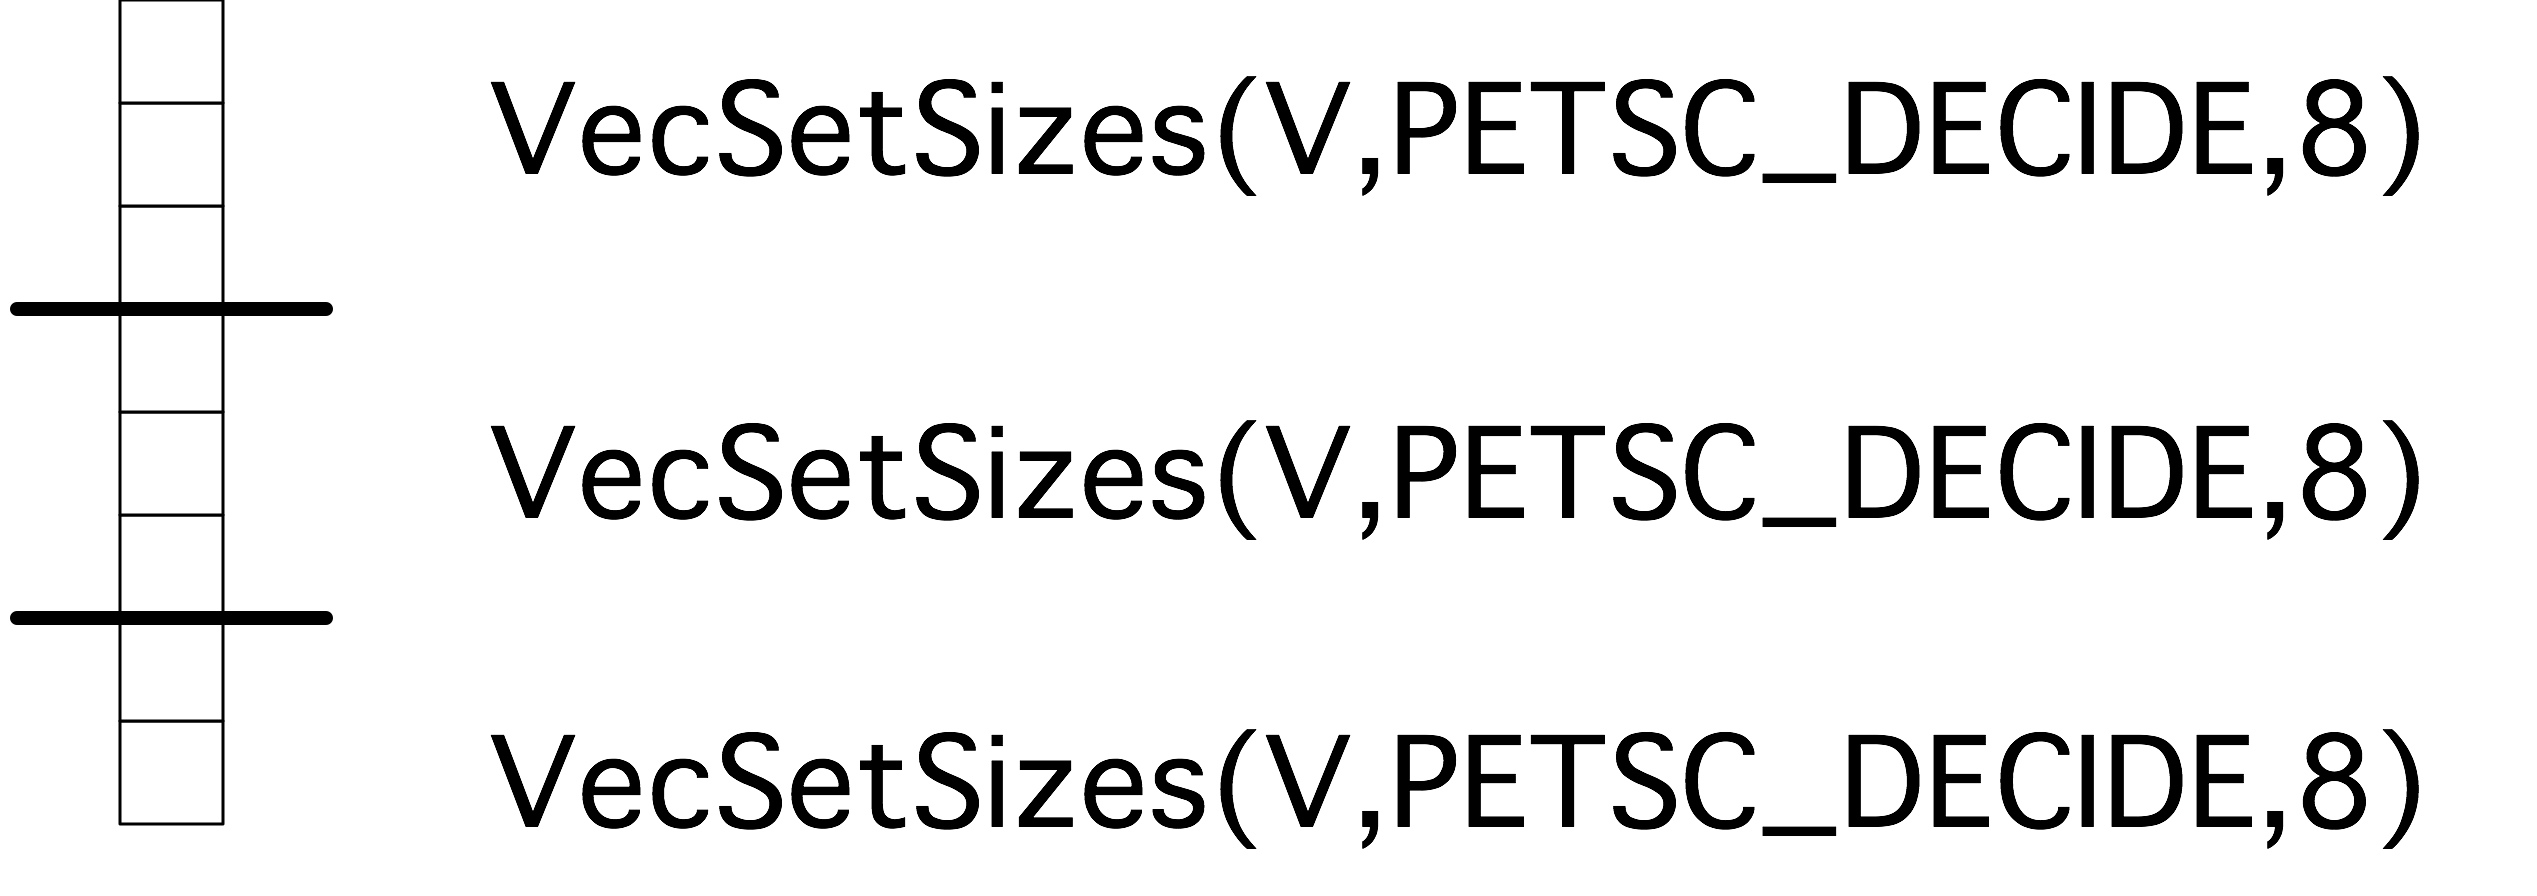
\includegraphics[scale=.08]{veccreate2}
}

\frame[containsverbatim]{\frametitle{Parallel layout specified}
Local or global size in
\begin{verbatim}
VecSetSizes(Vec v, int m, int M);
\end{verbatim}
Global size can be specified as \n{PETSC_DECIDE}.

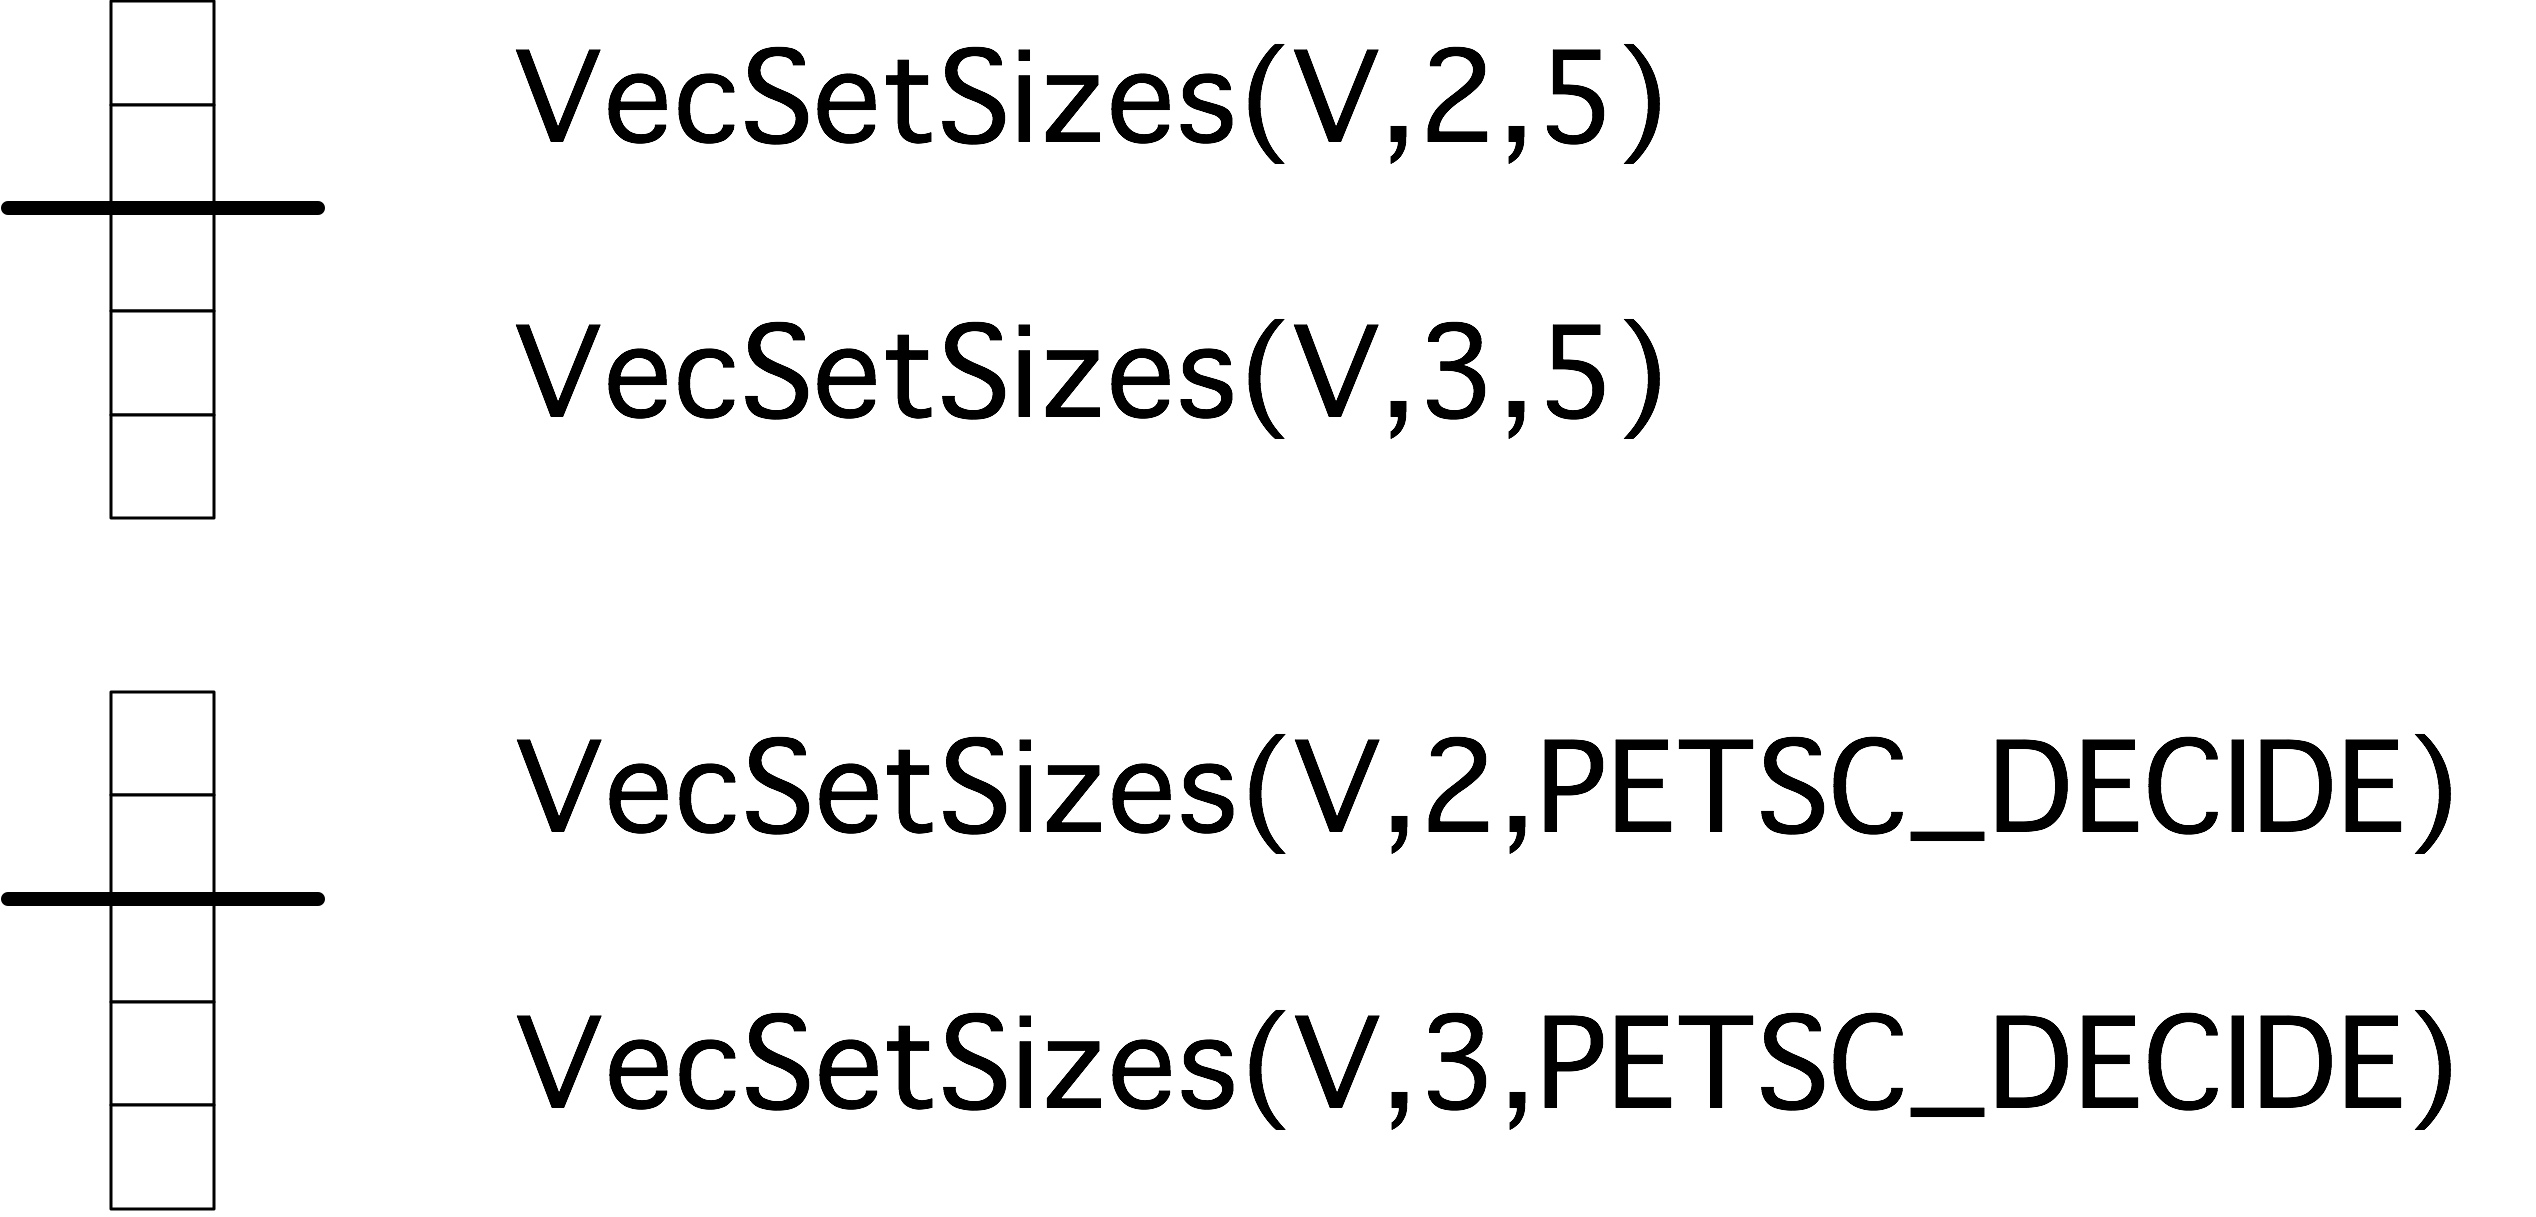
\includegraphics[scale=.08]{veccreate1}
}

\begin{details}
\frame[containsverbatim]{\frametitle{Query parallel layout}
Query vector layout:
\begin{verbatim}
VecGetSize(Vec,PetscInt *globalsize)
VecGetLocalSize(Vec,PetscInt *localsize)
VecGetOwnershipRange(Vec x,PetscInt *low,PetscInt *high)
VecGetOwnershipRange(x,low,high,ierr) ! F
\end{verbatim}
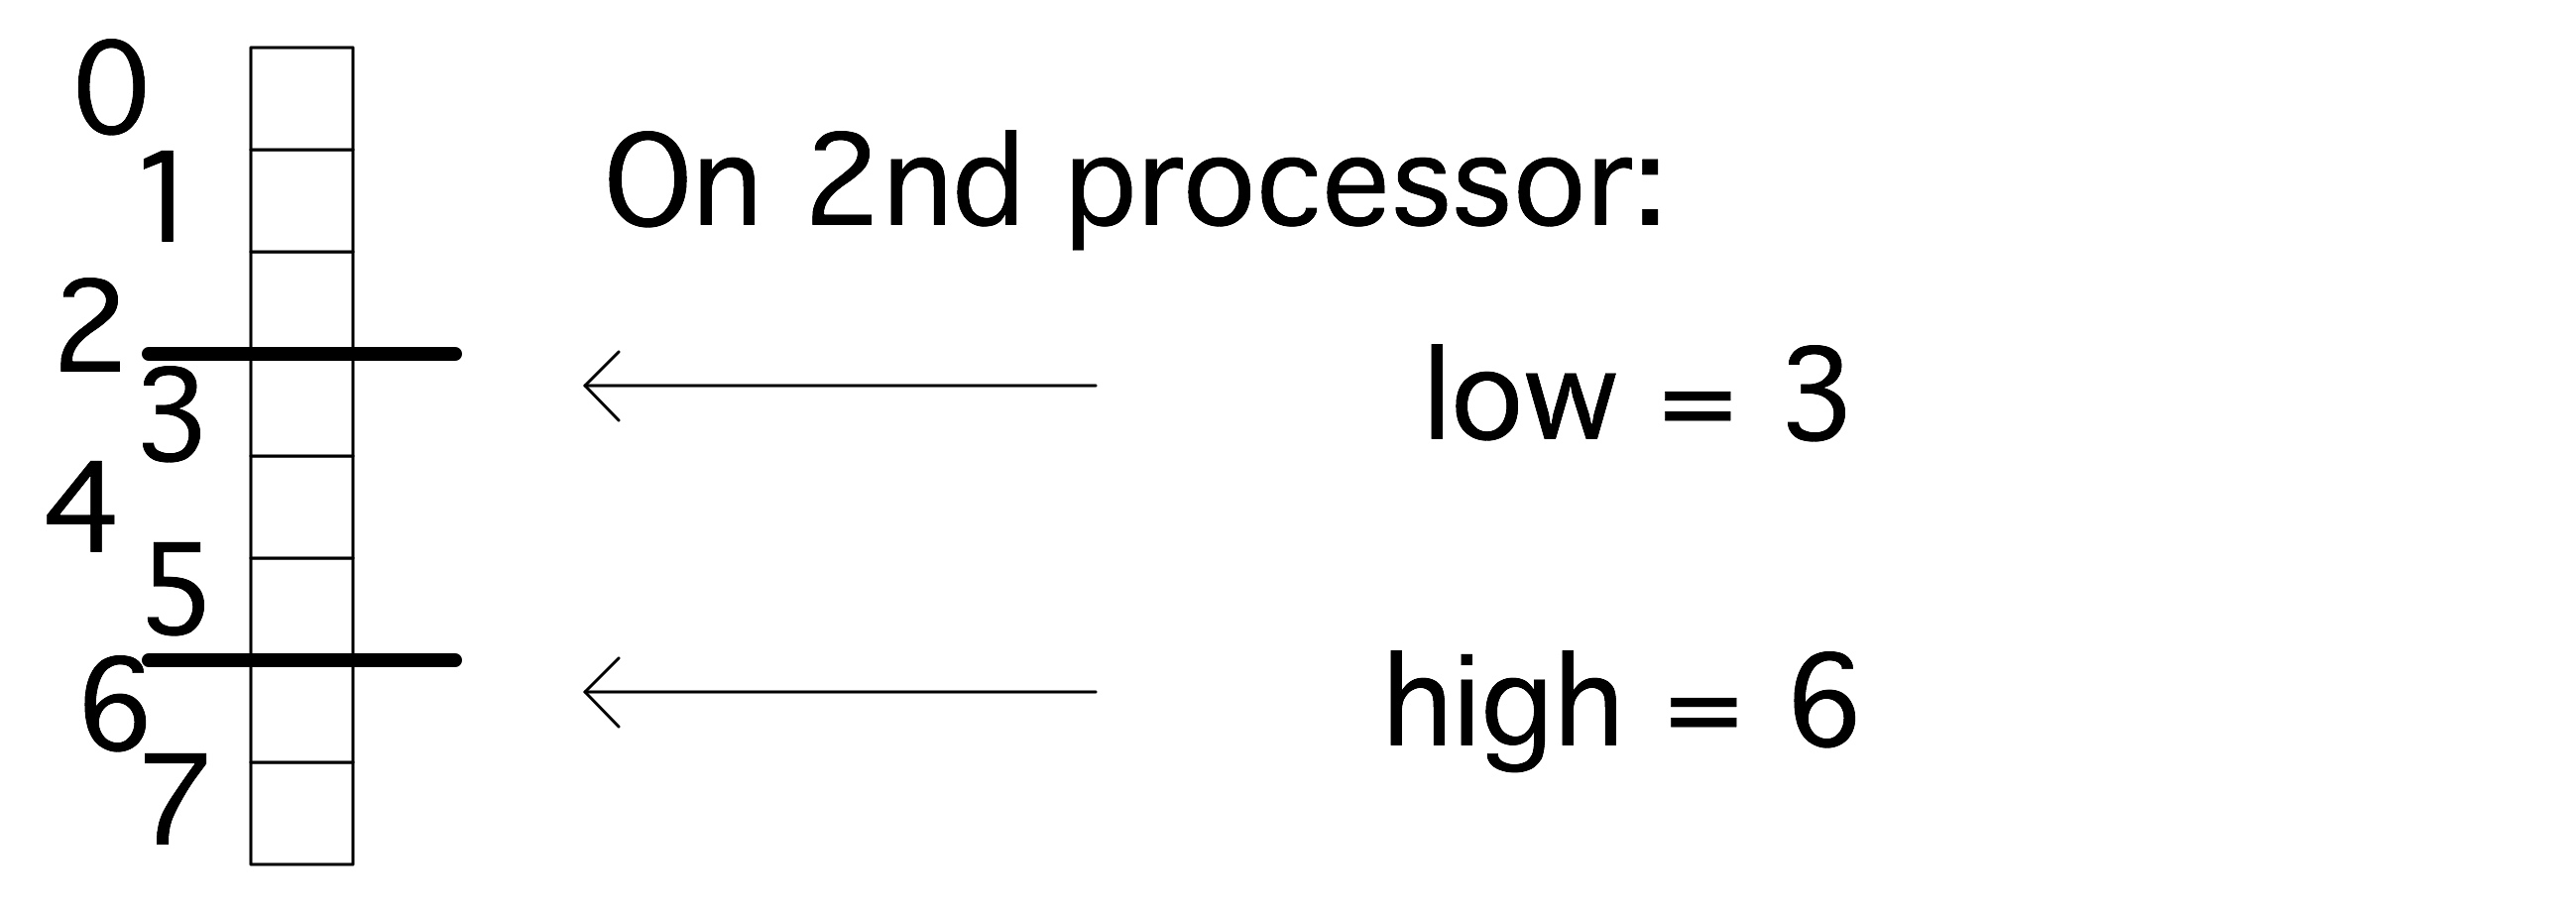
\includegraphics[scale=.08]{veclayout}

Query general layout:
\begin{verbatim}
PetscSplitOwnership(MPI_Comm comm,PetscInt *n,PetscInt *N);
PetscSplitOwnership(comm,n,N,ierr) ! F
\end{verbatim}
(get local/global given the other)
}
\end{details}

\frame[containsverbatim]{\frametitle{Setting values}
\small
Set vector to constant value:
\begin{verbatim}
VecSet(Vec x,PetscScalar value);
\end{verbatim}
Set individual elements (global indexing!):
\begin{verbatim}
VecSetValue(Vec x,int row,PetscScalar value, InsertMode mode);

i = 1; v = 3.14;
VecSetValue(x,i,v,INSERT_VALUES);

call VecSetValue(x,i,v,INSERT_VALUES,ierr,e)
\end{verbatim}
}

\frame[containsverbatim]{\frametitle{Setting values by block}
Set individual elements (global indexing!):
\begin{verbatim}
VecSetValues(Vec x,int n,int *rows,PetscScalar *values,
    InsertMode mode); // INSERT_VALUES or ADD_VALUES

ii[0] = 1; ii[1] = 2; vv[0] = 2.7; vv[1] = 3.1;
VecSetValues(x,2,ii,vv,INSERT_VALUES);

ii(1) = 1; ii(2) = 2; vv(1) = 2.7; vv(2) = 3.1
call VecSetValues(x,2,ii,vv,INSERT_VALUES,ierr,e)
\end{verbatim}
}

\frame[containsverbatim]{\frametitle{Setting values}
No restrictions on parallelism;\\
after setting, move values to appropriate processor:
\begin{verbatim}
VecAssemblyBegin(Vec x);
VecAssemblyEnd(Vec x);
\end{verbatim}
}

\frame[containsverbatim]{\frametitle{Basic operations}
\small
\begin{verbatim}
VecAXPY(Vec y,PetscScalar a,Vec x);   /* y <- y + a x */
VecAYPX(Vec y,PetscScalar a,Vec x);   /* y <- a y + x */
VecScale(Vec x, PetscScalar a);
VecDot(Vec x, Vec y, PetscScalar *r); /* several variants */
VecMDot(Vec x,int n,Vec y[],PetscScalar *r);
VecNorm(Vec x,NormType type, double *r);
VecSum(Vec x, PetscScalar *r);
VecCopy(Vec x, Vec y);
VecSwap(Vec x, Vec y);
VecPointwiseMult(Vec w,Vec x,Vec y);
VecPointwiseDivide(Vec w,Vec x,Vec y);
VecMAXPY(Vec y,int n, PetscScalar *a, Vec x[]);
VecMax(Vec x, int *idx, double *r);
VecMin(Vec x, int *idx, double *r);
VecAbs(Vec x);
VecReciprocal(Vec x);
VecShift(Vec x,PetscScalar s);
\end{verbatim}
}

\begin{exerciseframe}[vec]
Use the routines \n{VecDot}, \n{VecScale} and \n{VecNorm} to
compute the inner product of vectors \n{x,y}, scale the vector~\n{x},
and check its norm:
\[
\begin{array}{l}
p \leftarrow x^ty\\
x \leftarrow x/p\\
n \leftarrow \|x\|_2\\
\end{array}
\]
\end{exerciseframe}

\begin{details}
\frame[containsverbatim]{\frametitle{Getting values (C)}
\small
 Setting values is done without user access to the stored data\\
 Getting values is often not necessary: many operations provided.\\
what if you do want access to the data?
  \begin{itemize}
  \item Create vector from user provided array:
\begin{verbatim}
VecCreateSeqWithArray(MPI_Comm comm,
  PetscInt n,const PetscScalar array[],Vec *V)
VecCreateMPIWithArray(MPI_Comm comm,
  PetscInt n,PetscInt N,const PetscScalar array[],Vec *vv)
\end{verbatim}
\item Get the internal array (local only; see \n{VecScatter} for more general
  mechanism):
\begin{verbatim}
VecGetArray(Vec x,PetscScalar *a[])
/* do something with the array */
VecRestoreArray(Vec x,PetscScalar *a[])
\end{verbatim}
  \end{itemize}
}

\frame[containsverbatim]{\frametitle{Getting values example}
\begin{verbatim}
int localsize,first,i;
PetscScalar *a;
VecGetLocalSize(x,&localsize);
VecGetOwnershipRange(x,&first,PETSC_NULL);
VecGetArray(x,&a);
for (i=0; i<localsize; i++)
  printf("Vector element %d : %e\n",first+i,a[i]);
VecRestoreArray(x,&a);
\end{verbatim}
Fortran: \n{PETSC_NULL_INTEGER}
}

\frame[containsverbatim]{\frametitle{Array handling in F90}
\begin{verbatim}
    PetscScalar, pointer :: xx_v(:)
    ....
    call VecGetArrayF90(x,xx_v,ierr)
    a = xx_v(3)
    call VecRestoreArrayF90(x,xx_v,ierr)
\end{verbatim}
More seperate F90 versions for `Get' routines\\
(there are some ugly hacks for F77)
}
\end{details}

